\clearpage

\section{Experimental Setup}
\label{cp6:procedures}


% TODO ---- problematic


Our experiment's main hypothesis is that:


\medskip
\begin{bluequote}
    \textit{text automatically identified by a semantic-based technique assists a 
    developer complete her software development task.} 
\end{bluequote}



To test this hypothesis, we detail a controlled experiment where participants
 had to complete two programming tasks when assisted (or not) by a
 tool that embeds one of the best performing semantic-based techniques that we have explored previously ({Section~\ref{cp5:results-all}). 


We first evaluate how the text that a participant manually identifies as relevant (while she performs a task) 
compares to text that an automatic technique identifies. 
We then consider if a participant found the text automatically identified helpful, i.e., the text identified provides useful information needed to correctly complete her task.


In the following sections, we detail our experimental setup.


\art{Add a figure to help summarizing the experimental setup?}






\subsection{Design}


We follow a \textit{within-subjects} design. Each participant is exposed to a control task and a tool assisted task. For each of these tasks, we provided to the participants a set of natural language artifacts related to the task
and we asked them to code a solution for the task. While tasks were randomly assigned to each participant, 
we ensured that the tasks were evenly distributed among control and tool assisted groups. 






\subsection{Participants}



We advertised our study to both professionals in our personal network and to Computer Science students at the University of British Columbia. 
This provides for breadth of experience where novice and expert developers attempt our the tasks that we have selected. 


We advertised the study only to third and fourth-year students to ensure that they had the necessary background required to perform the study's taks.
At this point in the curriculum, they should be familiar with Python and they should be able to come up with a solution 
for a software task when provided with artifacts containing information for that task.


Participants were offered the opportunity to enter a raffle for one of two iPads 64 GB.




\subsection{Tasks}


Our experiment requires programming tasks for which a developer will likely benefit from the use of additional information to complete. We also need to ensure that the tasks are enough self-contained so that they can be finished in a single experimental session. These criteria lead us to 
follow Thiselton and Treude's task selection procedures~\cite{thiselton2019}, 
i.e., we select tasks from the Python w3resource website\footnote{\url{https://www.w3resource.com/python-exercises/}}
that require using at least one module external to the Python core modules. 



Table~\ref{tbl:python-tasks-modules} details the tasks and modules that we have selected. These tasks focus on modules that have been widely used.
For example, Reddit---a social news aggregator with approximately 430 million monthly users---uses the \texttt{BS4} module
to parse 
urls and identify images shown on its posts' headlines~\cite{bs4-reddit} while SquareUp---a digital  payments company---uses \texttt{pandas} for data analysis. 


% \footnote{\url{https://www.crummy.com/software/BeautifulSoup/}} 


\art{Add table with tasks.}





\subsection{Coding Environment}


To ensure that participants had the same conditions, we used Google Colab\footnote{\url{https://colab.research.google.com/}} as our coding environment. 
By using Colab, we expect setup instructions to be minimal 
so that we allow a participant to focus on the task-at-hand.



Figure~\ref{fig:online-judge} shows the \texttt{NYTimes} task (left-hand side) and its Colab environment (right-hand side). 
Participants had the task description and examples of input and output scenarios for the task as well as the resources associated with that task. 
Colab provided a code editor with amenities commonly found in modern IDEs, such as code completion and syntax highlighting. 

Through Colab, a participant could compile their solution and test it against the examples shown alongside the task description.
Upon testing, the system would display full details about the test cases, e.g., the test's input, which assertion failed, and why. 


 
\clearpage

\begin{landscape}
\begin{figure}
    \centering
    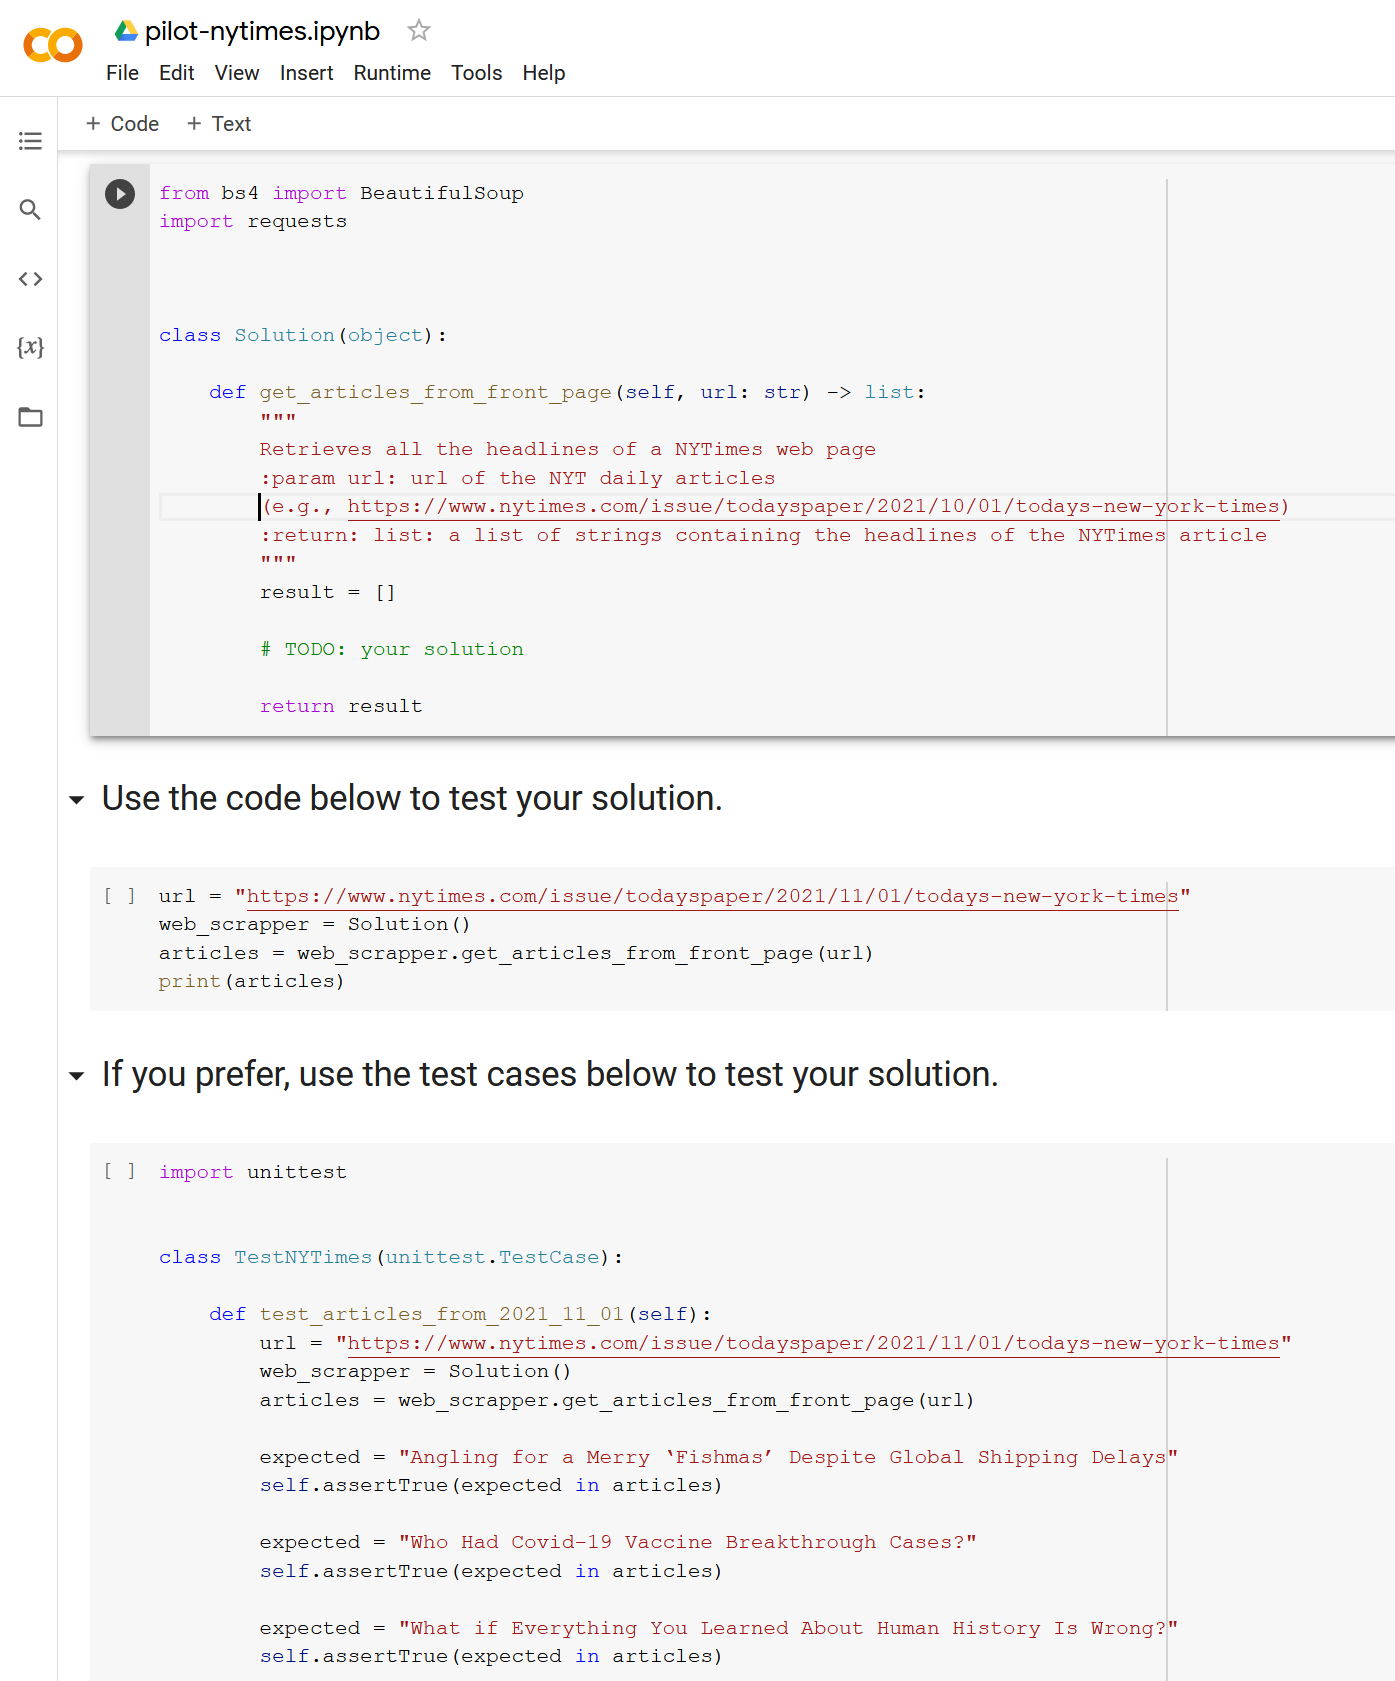
\includegraphics[width=\textwidth]{cp6/colab.png}
    \caption{Tasks and Colab environment.}
    \label{fig:nytimes}
\end{figure}
\end{landscape}

\clearpage



\subsubsection{Procedures}
\label{cp6:evaluation-procedures}


Each experimental session lasted no more than two hours; this length of time was selected based on two pilot sessions. 



We began each session gathering consent and requesting participants to install a web browser plugin which we used to gather data.
Setup was followed by a short tutorial explaining the experiment and describing how to use the plugin and Colab. 
A practice task, separated from the experimental tasks,
 allowed participants to familiarize themselves with the content of a task, the web browser plugin, and Colab. 




Participants were randomly assigned to a control task and to a tool assisted task, each.
For these tasks, participants were asked to inspect a set of artifacts with documentation related to that task and then, to write a solution for the task. 
In the control task, participants could use the web browser plugin to highlight any text that they deemed relevant to the task-at-hand. 
In the tool assisted task, the plugin automatically highlighted sentences that it identified as relevant for the task. 
For this second task, experimental procedures had one extra step asking a participant to rate---using a Likert scale---how helpful were the highlights automatically identified. 




\subsubsection{Analysis}


We use each task as our unit of analysis. For each tasks, we report dependent variables within groups (i.e., control and tool-assisted) and between groups (i.e., control \textit{vs} tool-assisted)



\clearpage



\smallskip
\paragraph{\textbf{Problems with Android/Java tasks:}}

\begin{itemize}
    \item Installing and running the Android SDK is not trivial
    \item The Android emulators consume too much memory and it may be difficult to perform the tasks in certain environments
    \item Most of the tasks are visual and they don't have easy test cases that I can use to provide feedback to the students
\end{itemize}



% \subsubsection{Tasks}

% We use bugs or feature requests obtained from three popular \red{Android} GitHub repos (i.e., \textit{Omni-Notes}, \textit{K-9}, and \textit{AntennaPod}) as the tasks of our experiment. 
% We manually inspected each of the pull requests merged to the master branch in these repos and selected issues that had changes in a single file and that are related to different components core to the Android API.
% This manual inspection lead us to select the following tasks:
% \footnote{
% \textcolor{steelblue}{{\textit{AM:} one challenge with Android tasks is that, while more representative, they are harder to debug and test in a self-contained environment.
% A potential alternative are Python tasks that require using well-known modules. https://www.practicepython.org/ has examples for \texttt{beautifulsoup}}}}.

% % ---\textit{Omni-Notes}, \textit{K-9}, and \textit{AntennaPod}---



% \begin{itemize}
%     \item \texttt{Notifications}: notify users about new emails in their inbox;
%     \item \texttt{Permissions}: request user permissions to and external storage; and
%     \item \texttt{Storage}: show size of all the data used by the application.
% \end{itemize}


% While these tasks are small enough so that a student can come up with a solution in a single programming session,
% they require understanding interactions between different API components 
% and likely require the students to seek information in the Android API documentation or in community forums. 
% Therefore, we deem the tasks as appropriate to a scenario where our tool could assist a student trying to find information relevant to these tasks in a set of natural language artifacts. 


% \subsubsection{Android Application}


% Ideally, all tasks could have been selected from the same open-source project. However, our requirements on the number of classes or methods in a task's solution as well as the need that the tasks relate to core Android API components made it difficult 
% to identify a single project with such self-contained tasks. Since asking a student to familiarize themselves with running, debugging and modifying three different and complex Android applications 
% poses challenge to experimental procedures, we decided to use the 2019 Google I/O Android demo application as the core project in which the selected tasks must be implemented. 
% % \footnote{\url{https://github.com/marquesarthur/iosched}}


% The I/O Android app displays a list of conference events---sessions, office hours, app reviews, codelabs, etc.---and it lets a user filter these events by event types and by topics.
% This project has \red{[statistics about number of classes, lines, etc.]} and we believe that we can transpose the tasks that we have selected to this Android app without loss of context or complexity. 
% That is, to perform each of the selected tasks, a developer still has to make changes to a single file and they still need to consult supporting material to identify information that guides them towards 
% a solution.





% We report metrics related to the text that participants in the experiment indicated as helpful to the task-at-hand, their agreement on the extent to which the text automatically identified by our tool 
% assisted them, and how complete were their solutions, as measured by test cases that judged
% their code.


%  TODO: easy part ???? more descriptive